

Identifying action instances in time and recognizing their categories, known as temporal action localization (TAL), remains a challenging problem in video understanding. Significant progress has been made in developing deep models for TAL. Most previous works have considered using action proposals~\cite{bmniccv2019} or anchor windows~\cite{gaussiancvpr2019}, and developed convolutional~\cite{ssniccv2017,cdc2017cvpr}, recurrent~\cite{sstadbmvc2017}, and graph~\cite{bcgnneccv2020,gtadcvpr2020,yang2022acgnet} neural networks for TAL. Despite a steady progress on major benchmarks, the accuracy of existing methods usually comes at a price of modeling complexity, with increasingly sophisticated proposal generation, anchor design, loss function, network architecture, and output decoding process.

\noindent\begin{wrapfigure}{l}{0.52\textwidth} 
	\centering
	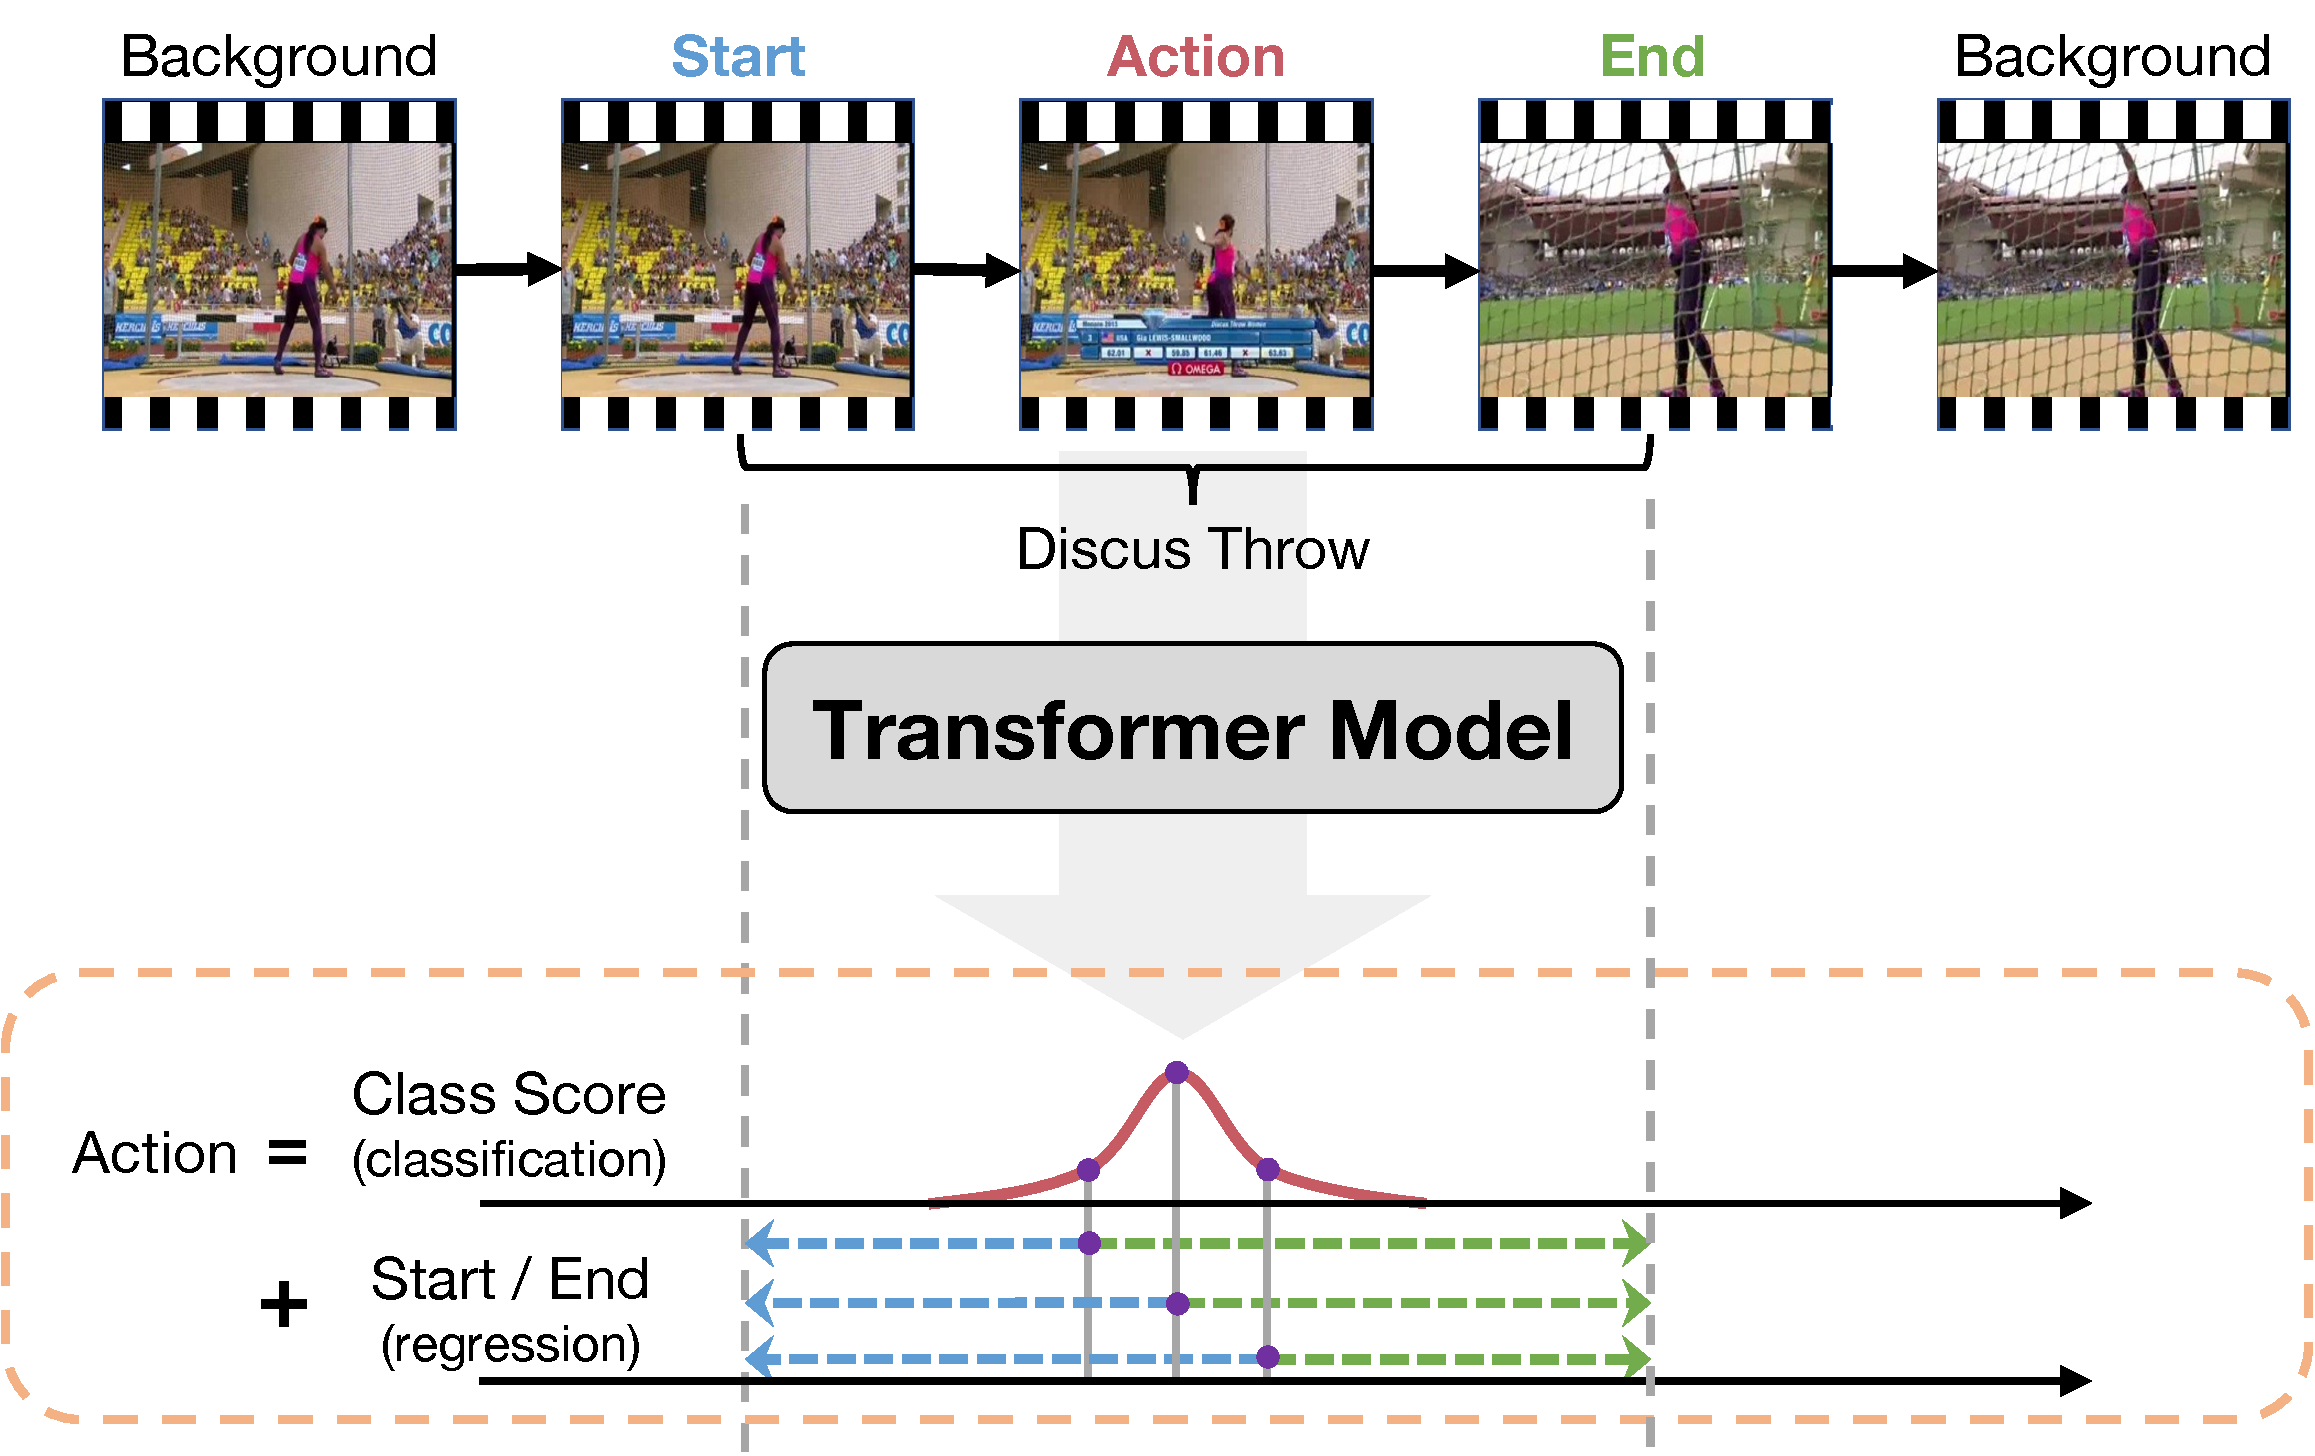
\includegraphics[width=0.95\linewidth]{figure/action_teaser_new.pdf}
	\caption{\textbf{An illustration of our ActionFormer}. We propose a Transformer based model to localize action instances in time (\emph{top}) by (1) classifying every moment into action categories and (2) estimating their distances to action boundaries (\emph{bottom}).}
	\label{fig:teaser}
\end{wrapfigure}%
In this paper, we adopt a minimalist design and develop a Transformer based model for TAL, inspired by the recent success of Transformers in NLP~\cite{transformernips2017,devlin2019bert} and vision~\cite{vitarxiv2020,swiniccv2021,detreccv2020}. Originally developed for sequence data, Transformers use self-attention to model long-range dependencies, and thus are a natural fit for TAL in untrimmed videos. Our method, illustrated in Fig.\ \ref{fig:teaser}, adapts local self-attention to model temporal context in an input untrimmed videos, classifies every moment, and regresses their corresponding action boundaries. The result is a deep model trained using standard classification and regression loss, and can localize moments of actions in a single shot, without using action proposals or pre-defined anchor windows. 

Specifically, our model, dubbed ActionFormer, integrates local self-attention to extract a feature pyramid from an input video. Each location in the output pyramid represents a moment in the video, and is treated as an action candidate. A lightweight convolutional decoder is further employed on the feature pyramid to classify these candidates into foreground action categories, and to regress the distance between a foreground candidate and its action onset and offset. The results can be easily decoded into actions with their labels and temporal boundaries. Our method thus provides a {\it single-stage anchor-free} model for TAL. 

We show that such a simple model, with proper design, can be surprisingly powerful for TAL. In particular, ActionFormer establishes a new state of the art across several major TAL benchmarks, surpassing previous works by a significant margin. For example, ActionFormer achieves 71.0\% \textit{m}AP at tIoU$=$0.5 on THUMOS14, outperforming the best prior model by 14.1 absolute percentage points. Further, ActionFormer reaches an average \textit{m}AP of 36.6\% on ActivityNet 1.3. More importantly, ActionFormer shows impressive results on EPIC-Kitchens 100 for egocentric action localization, with a boost of over 13.5 absolute percentage points in average \textit{m}AP. %

Our work is based on simple techniques, supported by favourable empirical results, and validated by extensive ablation experiments, at our best. Our main contributions are summarized as follows. First, we are among the first to propose a Transformer based model for single-stage anchor-free TAL. Second, we study key design choices of developing Transformer models for TAL, and demonstrate a simple model that works surprisingly well. Finally, our model achieves state-of-the-art results across major benchmarks and offers a solid baseline for TAL. 

